\documentclass{article}
\usepackage{amsmath}
\usepackage{amssymb}
\usepackage{tikz}
\usetikzlibrary{shapes.geometric}
\usepackage[T1]{fontenc}

\begin{document}

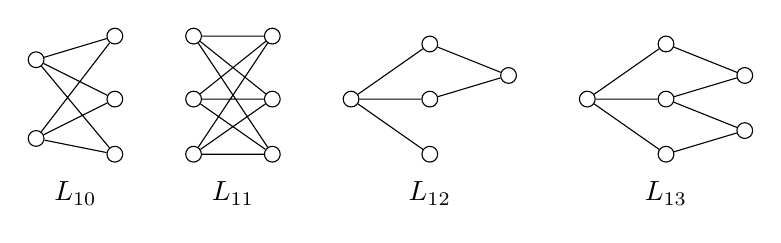
\begin{tikzpicture}[hhh/.style={draw=black,circle,inner sep=2pt,minimum size=0.2cm}]
		
		\begin{scope}[shift={(0,0)}]
			\node 	   (a) at (0,0) 		{$L_{10}$};
			\node[hhh] (b1) at (-0.5,0.7)	{};
			\node[hhh] (b2) at (-0.5,1.7)	{};
			\node[hhh] (c1) at (0.5,0.5) 		{};
			\node[hhh] (c2) at (0.5,1.2) 		{};
			\node[hhh] (c3) at (0.5,2) 		{};
			
			\draw (c1) -- (b1) (c2) -- (b1)  (c3) -- (b1)
			(c1) -- (b2) (c2) -- (b2)  (c3) -- (b2);
		\end{scope}
		
		\begin{scope}[shift={(2,0)}]
			\node 	   (a) at (0,0) 		{$L_{11}$};
			\node[hhh] (b1) at (-0.5,0.5)	{};
			\node[hhh] (b2) at (-0.5,1.2)	{};
			\node[hhh] (b3) at (-0.5,2)	{};
			\node[hhh] (c1) at (0.5,0.5) 		{};
			\node[hhh] (c2) at (0.5,1.2) 		{};
			\node[hhh] (c3) at (0.5,2) 		{};
			
			\draw (c1) -- (b1) (c2) -- (b1)  (c3) -- (b1)
			(c1) -- (b2) (c2) -- (b2)  (c3) -- (b2)
			(c1) -- (b3) (c2) -- (b3)  (c3) -- (b3);
		\end{scope}
		
		\begin{scope}[shift={(4.5,0)}]
			\node 	   (a) at (0,0) 		{$L_{12}$};
			\node[hhh] (b) at (-1,1.2)	{};
			\node[hhh] (c1) at (0,0.5) 		{};
			\node[hhh] (c2) at (0,1.2) 		{};
			\node[hhh] (c3) at (0,1.9) 		{};
			\node[hhh] (d) at (1,1.5) 	{};
			
			\draw (c1) -- (b) (c2) -- (b)  (c3) -- (b) (c2)--(d)--(c3);
		\end{scope}
		
		\begin{scope}[shift={(7.5,0)}]
			\node 	   (a) at (0,0) 		{$L_{13}$};
			\node[hhh] (b) at (-1,1.2)	{};
			\node[hhh] (c1) at (0,0.5) 		{};
			\node[hhh] (c2) at (0,1.2) 		{};
			\node[hhh] (c3) at (0,1.9) 		{};
			\node[hhh] (d1) at (1,1.5) 	{};
			\node[hhh] (d2) at (1,0.8) 	{};
			
			\draw (c1) -- (b) (c2) -- (b)  (c3) -- (b) 
			(c2)--(d1)--(c3) (c1)--(d2)--(c2);
		\end{scope}
		
	\end{tikzpicture}

\end{document}